\documentclass{standalone}

\usepackage{tikz}
\usetikzlibrary{automata,arrows, fit, backgrounds}
\usepackage[compat=1.1.0]{tikz-feynman}
\usepackage{xcolor}

\begin{document}
    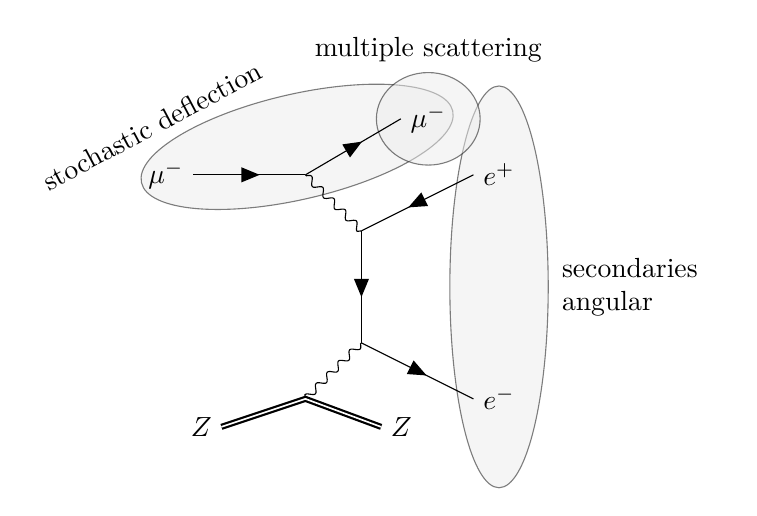
\begin{tikzpicture}
        % Sizes
        \pgfmathsetmacro{\len}{0.05cm}
        \pgfmathsetmacro{\halflen}{\len/4}
        \pgfmathsetmacro{\vertexsize}{\len/20}
        \begin{feynman}
            % vertices
            \vertex (a) at (0, 0);
            \vertex (b) at (0, -1*\len);
            \vertex (d) at (-0.5*\len, 0.5*\len);
            \vertex (c) at (-0.5*\len, -1.5*\len);
            \vertex (i1) at (-1.5*\len, 0.5*\len);
            \vertex (i2) at (0, 1.5*\len);
            \vertex (f1) at (\len, 0.5*\len);
            \vertex (f2) at (\len, -1.5*\len);
            \vertex (f3) at (0.5, 1*\len);
            \vertex (z1) at (-1.25*\len, -1.75*\len);
            \vertex (z2) at (0.25, -1.75*\len);

            % draw diagram
            \diagram* {
                (i1) -- [fermion] (d) -- [fermion] (f3),
                (d) -- [boson] (a),
                (f1) -- [fermion] (a),
                (a) -- [fermion] (b),
                (b) -- [fermion] (f2),
                (b) -- [boson] (c),
            };
            \draw[thick, double] (z1) -- (c) -- (z2);

            % labels
            \node[left] (I1) at (i1) {$\mu^-$};
            \node[right] (F3) at (f3) {$\mu^-$};
            \node[right] (F1) at (f1) {$e^+$};
            \node[right] (F2) at (f2) {$e^-$};
            \node[left] at (z1) {$Z$};
            \node[right] at (z2) {$Z$};
        \end{feynman}

    \begin{scope}[on background layer]
        \node [draw=black, fill=gray!15, ellipse, rotate=13, fit=(i1) (f3), opacity=0.5] (st) {};
        \node [draw=black, fill=gray!15, ellipse, fit=(F1) (F2), opacity=0.5]
            (sec){};
        \node [draw=black, fill=gray!15, ellipse, fit=(F3),opacity=0.5 ] (ms) {};

        \node [rotate=28, yshift=1.1cm, xshift=-1.5cm] at (st) {stochastic deflection};
        \node [above, yshift=0.6cm] at (ms) {multiple scattering};
        \node [xshift=1.8cm, text width=2cm] at (sec) {secondaries angular};
    \end{scope}

    \end{tikzpicture}
\end{document}
